%%%% Paramétrage du TD %%%%
\def\xxactivite{Activation 2 \ifprof -- Corrigé \else \fi} % \normalsize \vspace{-.4cm}
\def\xxauteur{\textsl{Xavier Pessoles}}

\def\xxnumchapitre{Chapitre 3 \vspace{.2cm}}
\def\xxchapitre{\hspace{.12cm} Application du Principe Fondamental de la Dynamique}

\def\xxtitreexo{Éolienne}
\def\xxsourceexo{\hspace{.2cm} \footnotesize{Émilien Durif}}
%\def\xxauteur{\textsl{Xavier Pessoles}}


\def\xxcompetences{%
\vspace{-.5cm}
\textsl{%
\textbf{Savoirs et compétences :}
\begin{itemize}[label=\ding{112},font=\color{ocre}] 
%\item \textit{Mod2.C16} : torseur cinétique
%\item \textit{Mod2.C17} : torseur dynamique
\item \textit{Mod2.C17.SF1} : déterminer le torseur dynamique d’un solide, ou d’un ensemble de solides, par rapport à un autre solide
%\item \textit{Mod2.C15} : matrice d'inertie
\item \textit{Res1.C2} : principe fondamental de la dynamique
%\item \textit{Res1.C1.SF1} : proposer une démarche permettant la détermination de la loi de mouvement
%\item \textit{Res1.C2.SF1} : proposer une méthode permettant la détermination d’une inconnue de liaison
\end{itemize}
}}
\def\xxfigures{
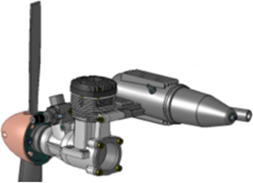
\includegraphics[width=.7\linewidth]{fig_00}}%figues de la page de garde


\iflivret
\pagestyle{empty}


%%%%%%%% PAGE DE GARDE COURS
\ifcours
% ==== BANDEAU DES TITRES ==== 
\begin{tikzpicture}[remember picture,overlay]
\node at (current page.north west)
{\begin{tikzpicture}[remember picture,overlay]
\node[anchor=north west,inner sep=0pt] at (0,0) {\includegraphics[width=\paperwidth]{\thechapterimage}};
\draw[anchor=west] (-2cm,-8cm) node [line width=2pt,rounded corners=15pt,draw=ocre,fill=white,fill opacity=0.6,inner sep=40pt]{\strut\makebox[22cm]{}};
\draw[anchor=west] (1cm,-8cm) node {\huge\sffamily\bfseries\color{black} %
\begin{minipage}{1cm}
\rotatebox{90}{\LARGE\sffamily\textsc{\color{ocre}\textbf{\xxnumpartie}}}
\end{minipage} \hfill
\begin{minipage}[c]{14cm}
\begin{titrepartie}
\begin{flushright}
\renewcommand{\baselinestretch}{1.1} 
\Large\sffamily\textsc{\textbf{\xxpartie}}
\renewcommand{\baselinestretch}{1} 
\end{flushright}
\end{titrepartie}
\end{minipage} \hfill
\begin{minipage}[c]{3.5cm}
{\large\sffamily\textsc{\textbf{\color{ocre} \discipline}}}
\end{minipage} 
 };
\end{tikzpicture}};
\end{tikzpicture}
% ==== FIN BANDEAU DES TITRES ==== 


% ==== ONGLET 
\begin{tikzpicture}[overlay]
\node[shape=rectangle, 
      rounded corners = .25 cm,
	  draw= ocre,
	  line width=2pt, 
	  fill = ocre!10,
	  minimum width  = 2.5cm,
	  minimum height = 3cm,] at (18.3cm,0) {};
\node at (17.7cm,0) {\rotatebox{90}{\textbf{\Large\color{ocre}{\classe}}}};
%{};
\end{tikzpicture}
% ==== FIN ONGLET 


\vspace{3.5cm}

\begin{tikzpicture}[remember picture,overlay]
\draw[anchor=west] (-2cm,-6cm) node {\huge\sffamily\bfseries\color{black} %
\begin{minipage}{2cm}
\begin{center}
\LARGE\sffamily\textsc{\color{ocre}\textbf{\xxactivite}}
\end{center}
\end{minipage} \hfill
\begin{minipage}[c]{15cm}
\begin{titrechapitre}
\renewcommand{\baselinestretch}{1.1} 
\Large\sffamily\textsc{\textbf{\xxnumchapitre}}

\Large\sffamily\textsc{\textbf{\xxchapitre}}
\vspace{.5cm}

\renewcommand{\baselinestretch}{1} 
\normalsize\normalfont
\xxcompetences
\end{titrechapitre}
\end{minipage}  };
\end{tikzpicture}
\vfill

\begin{flushright}
\begin{minipage}[c]{.3\linewidth}
\begin{center}
\xxfigures
\end{center}
\end{minipage}\hfill
\begin{minipage}[c]{.6\linewidth}
\startcontents
%\printcontents{}{1}{}
\printcontents{}{1}{}
\end{minipage}
\end{flushright}

\begin{tikzpicture}[remember picture,overlay]
\draw[anchor=west] (4.5cm,-.7cm) node {
\begin{minipage}[c]{.2\linewidth}
\begin{flushright}

\includegraphics[width=2cm]{logoCC}
\end{flushright}
\end{minipage}
\begin{minipage}[c]{.2\linewidth}
\textsl{\xxauteur} \\
\textsl{\classe}
\end{minipage}
 };
\end{tikzpicture}

\newpage
\pagestyle{fancy}

%\newpage
%\pagestyle{fancy}

\else
\fi
%% FIN PAGE DE GARDE DES COURS

%%%%%%%% PAGE DE GARDE TD
\iftd
%\begin{tikzpicture}[remember picture,overlay]
%\node at (current page.north west)
%{\begin{tikzpicture}[remember picture,overlay]
%\draw[anchor=west] (-2cm,-3.25cm) node [line width=2pt,rounded corners=15pt,draw=ocre,fill=white,fill opacity=0.6,inner sep=40pt]{\strut\makebox[22cm]{}};
%\draw[anchor=west] (1cm,-3.25cm) node {\huge\sffamily\bfseries\color{black} %
%\begin{minipage}{1cm}
%\rotatebox{90}{\LARGE\sffamily\textsc{\color{ocre}\textbf{\xxnumpartie}}}
%\end{minipage} \hfill
%\begin{minipage}[c]{13.5cm}
%\begin{titrepartie}
%\begin{flushright}
%\renewcommand{\baselinestretch}{1.1} 
%\Large\sffamily\textsc{\textbf{\xxpartie}}
%\renewcommand{\baselinestretch}{1} 
%\end{flushright}
%\end{titrepartie}
%\end{minipage} \hfill
%\begin{minipage}[c]{3.5cm}
%{\large\sffamily\textsc{\textbf{\color{ocre} \discipline}}}
%\end{minipage} 
% };
%\end{tikzpicture}};
%\end{tikzpicture}

%%%%%%%%%% PAGE DE GARDE TD %%%%%%%%%%%%%%%
%\begin{tikzpicture}[overlay]
%\node[shape=rectangle, 
%      rounded corners = .25 cm,
%	  draw= ocre,
%	  line width=2pt, 
%	  fill = ocre!10,
%	  minimum width  = 2.5cm,
%	  minimum height = 2.5cm,] at (18.5cm,0) {};
%\node at (17.7cm,0) {\rotatebox{90}{\textbf{\Large\color{ocre}{\classe}}}};
%%{};
%\end{tikzpicture}

% PARTIE ET CHAPITRE
%\begin{tikzpicture}[remember picture,overlay]
%\draw[anchor=west] (-1cm,-2.1cm) node {\large\sffamily\bfseries\color{black} %
%\begin{minipage}[c]{15cm}
%\begin{flushleft}
%\xxnumchapitre \\
%\xxchapitre
%\end{flushleft}
%\end{minipage}  };
%\end{tikzpicture}

% BANDEAU EXO
\iflivret % SI LIVRET
\begin{tikzpicture}[remember picture,overlay]
\draw[anchor=west] (-2cm,-3.3cm) node {\huge\sffamily\bfseries\color{black} %
\begin{minipage}{5cm}
\begin{center}
\LARGE\sffamily\color{ocre}\textbf{\textsc{\xxactivite}}

\begin{center}
\xxfigures
\end{center}

\end{center}
\end{minipage} \hfill
\begin{minipage}[c]{12cm}
\begin{titrechapitre}
\renewcommand{\baselinestretch}{1.1} 
\large\sffamily\textbf{\textsc{\xxtitreexo}}

\small\sffamily{\textbf{\textit{\color{black!70}\xxsourceexo}}}
\vspace{.5cm}

\renewcommand{\baselinestretch}{1} 
\normalsize\normalfont
\xxcompetences
\end{titrechapitre}
\end{minipage}};
\end{tikzpicture}
\else % ELSE NOT LIVRET
\begin{tikzpicture}[remember picture,overlay]
\draw[anchor=west] (-2cm,-4.5cm) node {\huge\sffamily\bfseries\color{black} %
\begin{minipage}{5cm}
\begin{center}
\LARGE\sffamily\color{ocre}\textbf{\textsc{\xxactivite}}

\begin{center}
\xxfigures
\end{center}

\end{center}
\end{minipage} \hfill
\begin{minipage}[c]{12cm}
\begin{titrechapitre}
\renewcommand{\baselinestretch}{1.1} 
\large\sffamily\textbf{\textsc{\xxtitreexo}}

\small\sffamily{\textbf{\textit{\color{black!70}\xxsourceexo}}}
\vspace{.5cm}

\renewcommand{\baselinestretch}{1} 
\normalsize\normalfont
\xxcompetences
\end{titrechapitre}
\end{minipage}};
\end{tikzpicture}

\fi

\else   % FIN IF TD
\fi


%%%%%%%% PAGE DE GARDE FICHE
\iffiche
\begin{tikzpicture}[remember picture,overlay]
\node at (current page.north west)
{\begin{tikzpicture}[remember picture,overlay]
\draw[anchor=west] (-2cm,-2.25cm) node [line width=2pt,rounded corners=15pt,draw=ocre,fill=white,fill opacity=0.6,inner sep=40pt]{\strut\makebox[22cm]{}};
\draw[anchor=west] (1cm,-2.25cm) node {\huge\sffamily\bfseries\color{black} %
\begin{minipage}{1cm}
\rotatebox{90}{\LARGE\sffamily\textsc{\color{ocre}\textbf{\xxnumpartie}}}
\end{minipage} \hfill
\begin{minipage}[c]{14cm}
\begin{titrepartie}
\begin{flushright}
\renewcommand{\baselinestretch}{1.1} 
\large\sffamily\textsc{\textbf{\xxpartie} \\} 

\vspace{.2cm}

\normalsize\sffamily\textsc{\textbf{\xxnumchapitre -- \xxchapitre}}
\renewcommand{\baselinestretch}{1} 
\end{flushright}
\end{titrepartie}
\end{minipage} \hfill
\begin{minipage}[c]{3.5cm}
{\large\sffamily\textsc{\textbf{\color{ocre} \discipline}}}
\end{minipage} 
 };
\end{tikzpicture}};
\end{tikzpicture}

\iflivret
\begin{tikzpicture}[overlay]
\node[shape=rectangle, 
      rounded corners = .25 cm,
	  draw= ocre,
	  line width=2pt, 
	  fill = ocre!10,
	  minimum width  = 2.5cm,
	  minimum height = 2.5cm,] at (18.5cm,.5cm) {};
\node at (17.9cm,.5cm) {\rotatebox{90}{\textsf{\textbf{\large\color{ocre}{\classe}}}}};
%{};
\end{tikzpicture}
\else
\begin{tikzpicture}[overlay]
\node[shape=rectangle, 
      rounded corners = .25 cm,
	  draw= ocre,
	  line width=2pt, 
	  fill = ocre!10,
	  minimum width  = 2.5cm,
%	  minimum height = 2.5cm,] at (18.5cm,1.1cm) {};
	  minimum height = 2.5cm,] at (18.6cm,0.5cm) {};
\node at (18cm,0.5cm) {\rotatebox{90}{\textsf{\textbf{\large\color{ocre}{\classe}}}}};
%{};
\end{tikzpicture}

\fi

\else
\fi



\else
\pagestyle{empty}


%%%%%%%% PAGE DE GARDE COURS
\ifcours
% ==== BANDEAU DES TITRES ==== 
\begin{tikzpicture}[remember picture,overlay]
\node at (current page.north west)
{\begin{tikzpicture}[remember picture,overlay]
\node[anchor=north west,inner sep=0pt] at (0,0) {\includegraphics[width=\paperwidth]{\thechapterimage}};
\draw[anchor=west] (-2cm,-8cm) node [line width=2pt,rounded corners=15pt,draw=ocre,fill=white,fill opacity=0.6,inner sep=40pt]{\strut\makebox[22cm]{}};
\draw[anchor=west] (1cm,-8cm) node {\huge\sffamily\bfseries\color{black} %
\begin{minipage}{1cm}
\rotatebox{90}{\LARGE\sffamily\textsc{\color{ocre}\textbf{\xxnumpartie}}}
\end{minipage} \hfill
\begin{minipage}[c]{14cm}
\begin{titrepartie}
\begin{flushright}
\renewcommand{\baselinestretch}{1.1} 
\Large\sffamily\textsc{\textbf{\xxpartie}}
\renewcommand{\baselinestretch}{1} 
\end{flushright}
\end{titrepartie}
\end{minipage} \hfill
\begin{minipage}[c]{3.5cm}
{\large\sffamily\textsc{\textbf{\color{ocre} \discipline}}}
\end{minipage} 
 };
\end{tikzpicture}};
\end{tikzpicture}
% ==== FIN BANDEAU DES TITRES ==== 


% ==== ONGLET 
\begin{tikzpicture}[overlay]
\node[shape=rectangle, 
      rounded corners = .25 cm,
	  draw= ocre,
	  line width=2pt, 
	  fill = ocre!10,
	  minimum width  = 2.5cm,
	  minimum height = 3cm,] at (18.3cm,0) {};
\node at (17.7cm,0) {\rotatebox{90}{\textbf{\Large\color{ocre}{\classe}}}};
%{};
\end{tikzpicture}
% ==== FIN ONGLET 


\vspace{3.5cm}

\begin{tikzpicture}[remember picture,overlay]
\draw[anchor=west] (-2cm,-6cm) node {\huge\sffamily\bfseries\color{black} %
\begin{minipage}{2cm}
\begin{center}
\LARGE\sffamily\textsc{\color{ocre}\textbf{\xxactivite}}
\end{center}
\end{minipage} \hfill
\begin{minipage}[c]{15cm}
\begin{titrechapitre}
\renewcommand{\baselinestretch}{1.1} 
\Large\sffamily\textsc{\textbf{\xxnumchapitre}}

\Large\sffamily\textsc{\textbf{\xxchapitre}}
\vspace{.5cm}

\renewcommand{\baselinestretch}{1} 
\normalsize\normalfont
\xxcompetences
\end{titrechapitre}
\end{minipage}  };
\end{tikzpicture}
\vfill

\begin{flushright}
\begin{minipage}[c]{.3\linewidth}
\begin{center}
\xxfigures
\end{center}
\end{minipage}\hfill
\begin{minipage}[c]{.6\linewidth}
\startcontents
%\printcontents{}{1}{}
\printcontents{}{1}{}
\end{minipage}
\end{flushright}

\begin{tikzpicture}[remember picture,overlay]
\draw[anchor=west] (4.5cm,-.7cm) node {
\begin{minipage}[c]{.2\linewidth}
\begin{flushright}

\includegraphics[width=2cm]{logoCC}
\end{flushright}
\end{minipage}
\begin{minipage}[c]{.2\linewidth}
\textsl{\xxauteur} \\
\textsl{\classe}
\end{minipage}
 };
\end{tikzpicture}

\newpage
\pagestyle{fancy}

%\newpage
%\pagestyle{fancy}

\else
\fi
%% FIN PAGE DE GARDE DES COURS

%%%%%%%% PAGE DE GARDE TD
\iftd
%\begin{tikzpicture}[remember picture,overlay]
%\node at (current page.north west)
%{\begin{tikzpicture}[remember picture,overlay]
%\draw[anchor=west] (-2cm,-3.25cm) node [line width=2pt,rounded corners=15pt,draw=ocre,fill=white,fill opacity=0.6,inner sep=40pt]{\strut\makebox[22cm]{}};
%\draw[anchor=west] (1cm,-3.25cm) node {\huge\sffamily\bfseries\color{black} %
%\begin{minipage}{1cm}
%\rotatebox{90}{\LARGE\sffamily\textsc{\color{ocre}\textbf{\xxnumpartie}}}
%\end{minipage} \hfill
%\begin{minipage}[c]{13.5cm}
%\begin{titrepartie}
%\begin{flushright}
%\renewcommand{\baselinestretch}{1.1} 
%\Large\sffamily\textsc{\textbf{\xxpartie}}
%\renewcommand{\baselinestretch}{1} 
%\end{flushright}
%\end{titrepartie}
%\end{minipage} \hfill
%\begin{minipage}[c]{3.5cm}
%{\large\sffamily\textsc{\textbf{\color{ocre} \discipline}}}
%\end{minipage} 
% };
%\end{tikzpicture}};
%\end{tikzpicture}

%%%%%%%%%% PAGE DE GARDE TD %%%%%%%%%%%%%%%
%\begin{tikzpicture}[overlay]
%\node[shape=rectangle, 
%      rounded corners = .25 cm,
%	  draw= ocre,
%	  line width=2pt, 
%	  fill = ocre!10,
%	  minimum width  = 2.5cm,
%	  minimum height = 2.5cm,] at (18.5cm,0) {};
%\node at (17.7cm,0) {\rotatebox{90}{\textbf{\Large\color{ocre}{\classe}}}};
%%{};
%\end{tikzpicture}

% PARTIE ET CHAPITRE
%\begin{tikzpicture}[remember picture,overlay]
%\draw[anchor=west] (-1cm,-2.1cm) node {\large\sffamily\bfseries\color{black} %
%\begin{minipage}[c]{15cm}
%\begin{flushleft}
%\xxnumchapitre \\
%\xxchapitre
%\end{flushleft}
%\end{minipage}  };
%\end{tikzpicture}

% BANDEAU EXO
\iflivret % SI LIVRET
\begin{tikzpicture}[remember picture,overlay]
\draw[anchor=west] (-2cm,-3.3cm) node {\huge\sffamily\bfseries\color{black} %
\begin{minipage}{5cm}
\begin{center}
\LARGE\sffamily\color{ocre}\textbf{\textsc{\xxactivite}}

\begin{center}
\xxfigures
\end{center}

\end{center}
\end{minipage} \hfill
\begin{minipage}[c]{12cm}
\begin{titrechapitre}
\renewcommand{\baselinestretch}{1.1} 
\large\sffamily\textbf{\textsc{\xxtitreexo}}

\small\sffamily{\textbf{\textit{\color{black!70}\xxsourceexo}}}
\vspace{.5cm}

\renewcommand{\baselinestretch}{1} 
\normalsize\normalfont
\xxcompetences
\end{titrechapitre}
\end{minipage}};
\end{tikzpicture}
\else % ELSE NOT LIVRET
\begin{tikzpicture}[remember picture,overlay]
\draw[anchor=west] (-2cm,-4.5cm) node {\huge\sffamily\bfseries\color{black} %
\begin{minipage}{5cm}
\begin{center}
\LARGE\sffamily\color{ocre}\textbf{\textsc{\xxactivite}}

\begin{center}
\xxfigures
\end{center}

\end{center}
\end{minipage} \hfill
\begin{minipage}[c]{12cm}
\begin{titrechapitre}
\renewcommand{\baselinestretch}{1.1} 
\large\sffamily\textbf{\textsc{\xxtitreexo}}

\small\sffamily{\textbf{\textit{\color{black!70}\xxsourceexo}}}
\vspace{.5cm}

\renewcommand{\baselinestretch}{1} 
\normalsize\normalfont
\xxcompetences
\end{titrechapitre}
\end{minipage}};
\end{tikzpicture}

\fi

\else   % FIN IF TD
\fi


%%%%%%%% PAGE DE GARDE FICHE
\iffiche
\begin{tikzpicture}[remember picture,overlay]
\node at (current page.north west)
{\begin{tikzpicture}[remember picture,overlay]
\draw[anchor=west] (-2cm,-2.25cm) node [line width=2pt,rounded corners=15pt,draw=ocre,fill=white,fill opacity=0.6,inner sep=40pt]{\strut\makebox[22cm]{}};
\draw[anchor=west] (1cm,-2.25cm) node {\huge\sffamily\bfseries\color{black} %
\begin{minipage}{1cm}
\rotatebox{90}{\LARGE\sffamily\textsc{\color{ocre}\textbf{\xxnumpartie}}}
\end{minipage} \hfill
\begin{minipage}[c]{14cm}
\begin{titrepartie}
\begin{flushright}
\renewcommand{\baselinestretch}{1.1} 
\large\sffamily\textsc{\textbf{\xxpartie} \\} 

\vspace{.2cm}

\normalsize\sffamily\textsc{\textbf{\xxnumchapitre -- \xxchapitre}}
\renewcommand{\baselinestretch}{1} 
\end{flushright}
\end{titrepartie}
\end{minipage} \hfill
\begin{minipage}[c]{3.5cm}
{\large\sffamily\textsc{\textbf{\color{ocre} \discipline}}}
\end{minipage} 
 };
\end{tikzpicture}};
\end{tikzpicture}

\iflivret
\begin{tikzpicture}[overlay]
\node[shape=rectangle, 
      rounded corners = .25 cm,
	  draw= ocre,
	  line width=2pt, 
	  fill = ocre!10,
	  minimum width  = 2.5cm,
	  minimum height = 2.5cm,] at (18.5cm,.5cm) {};
\node at (17.9cm,.5cm) {\rotatebox{90}{\textsf{\textbf{\large\color{ocre}{\classe}}}}};
%{};
\end{tikzpicture}
\else
\begin{tikzpicture}[overlay]
\node[shape=rectangle, 
      rounded corners = .25 cm,
	  draw= ocre,
	  line width=2pt, 
	  fill = ocre!10,
	  minimum width  = 2.5cm,
%	  minimum height = 2.5cm,] at (18.5cm,1.1cm) {};
	  minimum height = 2.5cm,] at (18.6cm,0.5cm) {};
\node at (18cm,0.5cm) {\rotatebox{90}{\textsf{\textbf{\large\color{ocre}{\classe}}}}};
%{};
\end{tikzpicture}

\fi

\else
\fi



\fi
\setlength{\columnseprule}{.1pt}

\pagestyle{fancy}
\thispagestyle{plain}

\ifprof
\vspace{5.1cm}
\else
\vspace{5.2cm}
\fi

\def\columnseprulecolor{\color{ocre}}
\setlength{\columnseprule}{0.4pt} 

%%%%%%%%%%%%%%%%%%%%%%%

\setcounter{exo}{0}



\ifprof
\else
\begin{multicols}{2}
\fi

\ifprof
\else
On s'intéresse au cours de cet exercice à une éolienne bipale telle que représentée sur la figure ci-dessous. 
\begin{center}
\begin{tabular}{cc}
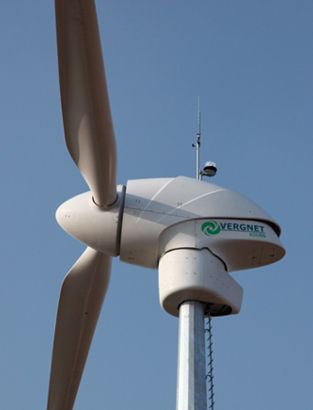
\includegraphics[width=0.35\linewidth]{eolienne_bipale.jpeg}
&
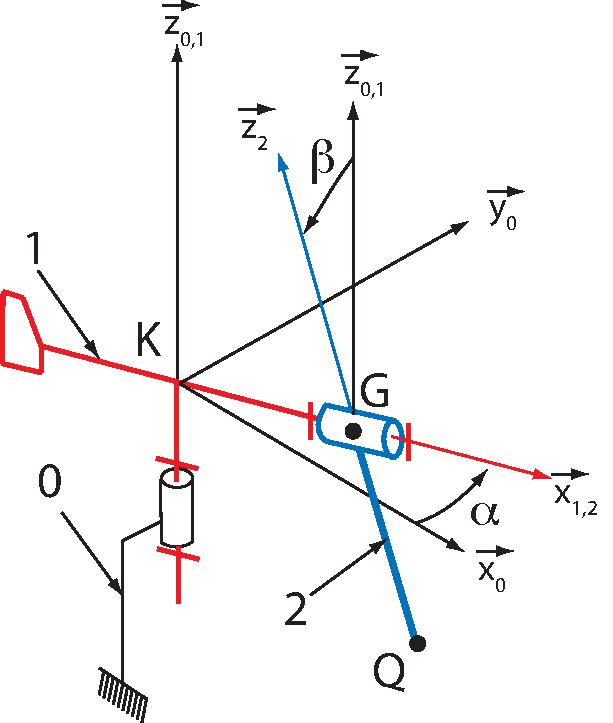
\includegraphics[width=0.55\linewidth]{eolienne.pdf}
\end{tabular}
\end{center}

Ce mécanisme est composé de trois ensembles en mouvement relatif que l'on décrit à l'aide de 4 solides.% (paramétrage) :
On cherche à dimensionner l'actionneur permettant l'orientation de l'éolienne lorsque les effets dynamiques d'un défaut de balourd sont prépondérants. 
%(diagramme des exigences partiel ci-dessous). 
%
%\begin{center}
%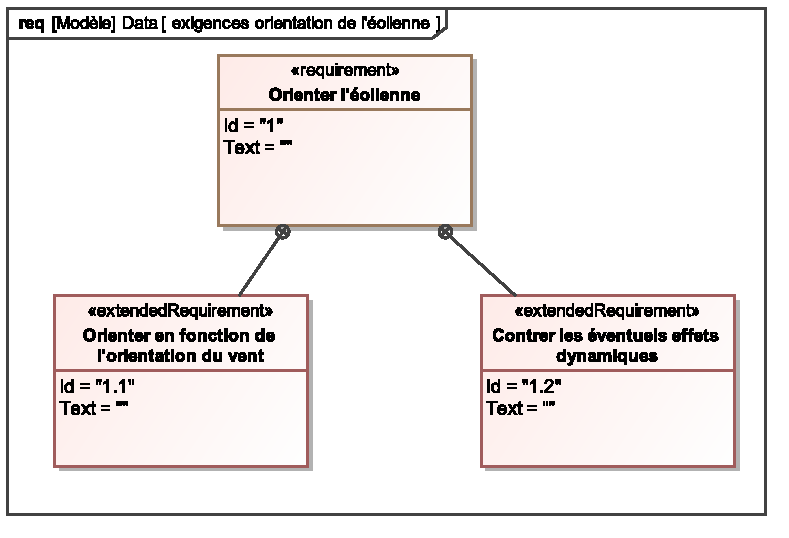
\includegraphics[width=\linewidth]{req_eolienne.pdf}
%\end{center}
On suppose donc que seule l'action mécanique due au moteur agissant entre $0$ et $1$ pour créer un couple $C_m$ selon la direction $\overrightarrow{z}_0$. 

L'éolienne est composée de : 
\begin{itemize}
\item un support \textbf{0}, auquel on associe un repère $R_0=\quadruplet{K}{\overrightarrow{x_0}}{\overrightarrow{y_0}}{\overrightarrow{z_0}}$;
\item une girouette \textbf{1} (de centre d'inertie $K$) en liaison pivot d'axe $\couple{K}{{z}_{0,1}}$ avec le support \textbf{0}. On lui associe un repère $R_1=\quadruplet{K}{\overrightarrow{x_1}}{\overrightarrow{y_1}}{\overrightarrow{z}_{0,1}}$ et on pose $\alpha=\couple{\overrightarrow{x_0}}{{x}_1}$. On note $J$ son moment d'inertie par rapport à l'axe $\couple{K}{{z}_1}$ : $J=I_{\couple{K}{{z}_1}}(1)$;
%\end{itemize}
\item une hélice \textbf{2}, en liaison pivot d'axe $\couple{K}{{x}_{1,2}}$  avec \textbf{1}. On lui associe un repère $R_2=\quadruplet{K}{\overrightarrow{x_{1,2}}}{\overrightarrow{y_2}}{\overrightarrow{z_2}}$  choisi tel que $\overrightarrow{x_2}=\overrightarrow{x_1}$ et on pose $\beta=\couple{\overrightarrow{y_1}}{{y}_2}$.
On note $M$ sa masse, $G$ son centre d'inertie situé sur l'axe de rotation et on pose $\overrightarrow{KG}=a\;\overrightarrow{x}_1$. On donne la matrice de l'opérateur d'inertie au point $G$ :
\begin{align*}
\overline{\overline{I}}_G(2)=
\left(
\begin{array}{ccc}
A & 0 & 0 \\ 
0 & B & 0 \\ 
0 & 0 & C
\end{array}
\right)_{\base{{x}_2}{{y}_2}{{z}_2}}.
\end{align*}
 

\item on modélise enfin un déséquilibre possible de l'hélice en rotation par un balourd \textbf{3} assimilé à une masse ponctuelle $m$ au point $Q$. On pose $\overrightarrow{GQ}=-b\overrightarrow{z_2}$.
\end{itemize}

\fi

\subparagraph{} \textit{Tracer le graphe de structure de l'éolienne.}
\ifprof
\begin{corrige}

\end{corrige}
\else
\fi


\subparagraph{} \textit{Déterminer le théorème à utiliser pour relier $C_m$ aux paramètres dynamiques du problème.}
\ifprof
\begin{corrige}
On pourra appliquer un théorème du moment dynamique s'appliquant sur l'éolienne ($E=\left\{1+2+3\right\}$) en projection sur l'axe $\couple{K}{{z}_0}$  : 
$\vectm{K}{\bar E}{E}\cdot \overrightarrow{z}_0=\vectmd{K}{E}{R_0}\cdot \overrightarrow{z}_0$
$\Leftrightarrow
C_m=\left(\vectmd{K}{1}{R_0}+\vectmd{K}{2}{R_0}+\vectmd{K}{3}{R_0}\right)\cdot \overrightarrow{z}_0$.
\end{corrige}
\else
\fi


\subparagraph{} \textit{Déterminer la composante suivant $\overrightarrow{z_0}$ du moment cinétique au point $K$ de la girouette \textbf{1} dans son mouvement par rapport au support \textbf{1}, notée $ \vectmc{K}{1}{0}\cdot\overrightarrow{z_0}$.}
\ifprof
\begin{corrige}
\begin{itemize}
\item Le mouvement de $1/0$ est un mouvement de rotation autour d'un axe fixe $\couple{K}{{z}_0}$ : 

\item $\vectmc{K}{1}{0}\cdot \overrightarrow{z}_0=\left(\overline{\overline{I}}_K(1)\cdot \overrightarrow{\Omega}(1/0)\right)\cdot \overrightarrow{z}_0=\left(\overline{\overline{I}}_K(1)\cdot \dot{\alpha}\cdot \overrightarrow{z}_0 \right)\cdot \overrightarrow{z}_0$

\item or on note $J$ son moment d'inertie par rapport à l'axe $\couple{K}{{z}}$ soit : 
$
\overline{\overline{I}}_K(1)\cdot\overrightarrow{z}_0\cdot \overrightarrow{z}_0=J
$

\item Ainsi : 
$
\vectmc{K}{1}{0}\cdot \overrightarrow{z}_0=J \dot{\alpha}
$.
\end{itemize}
\end{corrige}
\else
\fi


\subparagraph{} \textit{Déterminer le moment cinétique $\vectmc{K}{2}{0}$  calculé au point $K$ de l'hélice \textbf{2} dans son mouvement par rapport à \textbf{0}.}
\ifprof
\begin{corrige}
\begin{itemize}
\item Le mouvement de $2/0$ n'est pas un mouvement simple. 
\item On connaît l'opérateur d'inertie en $G$, on calcule donc : $\vectmc{G}{2}{0}$ :$
\vectmc{G}{2}{0}=\overline{\overline{I}}_G(2)\cdot \overrightarrow{\Omega}(2/0).$

\item On calcule $\overrightarrow{\Omega}(2/0)$ :
$\overrightarrow{\Omega}(2/0)=\overrightarrow{\Omega}(2/1)+\overrightarrow{\Omega}(1/0)$ 
$=\dot{\beta}\cdot \overrightarrow{x}_{1,2}+\dot{\alpha}\cdot \overrightarrow{z}_{1}$
$=\dot{\beta}\cdot \overrightarrow{x}_{1,2}
+\dot{\alpha}\left(\cos\beta\overrightarrow{z}_2+\sin\beta\overrightarrow{y}_2\right)$.

\item On calcule $\vectmc{G}{2}{0}$ : 
$
\vectmc{G}{2}{0}=\left(
\begin{array}{ccc}
A & 0 & 0 \\ 
0 & B & 0 \\ 
0 & 0 & C
\end{array}
\right)_{\base{{x}_2}{{y}_2}{{z}_2}} \cdot 
\left(
\begin{array}{c}
\dot{\beta}\\
\dot{\alpha}\cdot \sin\beta\\
\dot{\alpha}\cdot \cos\beta\\
\end{array}
\right)_{\base{{x}_2}{{y}_2}{{z}_2}}$
$=\left(
\begin{array}{c}
A\cdot \dot{\beta}\\
B\cdot \dot{\alpha}\cdot \sin\beta\\
C\cdot \dot{\alpha}\cdot \cos\beta\\
\end{array}
\right)_{\base{{x}_2}{{y}_2}{{z}_2}}.$

\item On calcule $\vectmc{K}{2}{0}$ : 
\begin{itemize}
\item $\vectmc{K}{2}{0}=\vectmc{G}{2}{0}+\overrightarrow{KG}\wedge \overrightarrow{R_c}(2/0)
=\vectmc{G}{2}{0}+a\cdot \overrightarrow{x}_1\wedge M\cdot \overrightarrow{V}(G\in 2/0)$
\item On calcule $\overrightarrow{V}(G\in 2/0)$ : 
$\overrightarrow{V}(G\in 2/0)=\overrightarrow{V}(K\in 2/0)+\overrightarrow{GK}\wedge \overrightarrow{\Omega}(2/0)=
\overrightarrow{0}-a\cdot \overrightarrow{x}_1\wedge \left(\dot{\beta}\cdot \overrightarrow{x}_{1,2}+\dot{\alpha}\cdot \overrightarrow{z}_{1}\right)\\
=a\cdot \dot{\alpha}\overrightarrow{y}_{1} $

\item On calcule $a\cdot \overrightarrow{x}_1\wedge M\cdot \overrightarrow{V}(G\in 2/0)$ : 
$
a\cdot \overrightarrow{x}_1\wedge M\cdot \overrightarrow{V}(G\in 2/0)=
a\cdot \overrightarrow{x}_1\wedge M\left(a\cdot \dot{\alpha}\overrightarrow{y}_{1} \right)=
M\cdot a^2\cdot \dot{\alpha}\cdot \overrightarrow{z}_1
$

\item On en déduit $\vectmc{K}{2}{0}$: $
\vectmc{K}{2}{0}=\left(
\begin{array}{c}
A\cdot \dot{\beta}\\
B\cdot \dot{\alpha}\cdot \sin\beta+M\cdot a^2\cdot \dot{\alpha}\sin\beta\\
C\cdot \dot{\alpha}\cdot \cos\beta+M\cdot a^2\cdot \dot{\alpha}\cos\beta\\
\end{array}
\right)_{\base{{x}_2}{{y}_2}{{z}_2}}\\
$
\end{itemize}
\end{itemize}
\end{corrige}
\else
\fi


\subparagraph{} \textit{Déterminer le moment cinétique $\vectmc{K}{3}{0}$}
\ifprof
\begin{corrige}
\begin{itemize}
\item Le solide $3$ est solide à masse ponctuelle, ainsi $\vectmc{Q}{3}{0}=\overrightarrow{0}$.
\item $\vectmc{K}{3}{0}=\overrightarrow{KQ}\wedge m\cdot \overrightarrow{V}(Q\in 3/0)$ : 
\begin{itemize}
\item On calcule $\overrightarrow{KQ}$ : 
$
\overrightarrow{KQ}=\overrightarrow{KG}+\overrightarrow{GQ}=a\cdot \overrightarrow{x}_1-b\cdot \overrightarrow{z}_2
$
\item On calcule $\overrightarrow{V}(Q\in 3/0)$ : 
$
\overrightarrow{V}(Q\in 3/0)=\overrightarrow{V}(Q\in 3/2)+\overrightarrow{V}(Q\in 2/1)+\overrightarrow{V}(Q\in 1/0)
$
$=\overrightarrow{0}+\overrightarrow{V}(G\in 2/1)+\overrightarrow{QG}\wedge \overrightarrow{\Omega}(2/1)
+\overrightarrow{V}(G\in 1/0)+\overrightarrow{QG}\wedge \overrightarrow{\Omega}(1/0)$
$=\overrightarrow{0}+b\cdot \overrightarrow{z}_2\wedge \dot{\beta}\cdot \overrightarrow{x}_2+ a\cdot \dot{\alpha}\cdot \overrightarrow{y}_1+b\cdot \overrightarrow{z}_2\wedge \dot{\alpha}\cdot \overrightarrow{z}_1$
$=b\cdot \dot{\beta}\cdot \overrightarrow{y}_2+a\cdot \dot{\alpha}\cdot \overrightarrow{y}_1-b\cdot\dot{\alpha} \sin\beta\cdot \overrightarrow{x}_{1,2}$


\item On calcule $\overrightarrow{KQ}\wedge m\overrightarrow{V}(Q\in 3/0)$ : 

$\overrightarrow{KQ}\wedge m\overrightarrow{V}(Q\in 3/0)=m\cdot \left[a\cdot \overrightarrow{x}_1-b\cdot \overrightarrow{z}_2\right]\wedge\left[b\cdot \dot{\beta}\cdot \overrightarrow{y}_2+a\cdot \dot{\alpha}\cdot \overrightarrow{y}_1-b\cdot\dot{\alpha} \sin\beta\cdot \overrightarrow{x}_{1,2}\right]$

$=m\left[a\cdot b\cdot \overrightarrow{z}_2+a^2\cdot \dot{\alpha}\cdot\overrightarrow{z}_1+b^2\cdot \dot{\beta}\cdot\overrightarrow{x}_2+b\cdot a\cdot \dot{\alpha}\cdot \cos\beta\cdot \overrightarrow{x}_1+b^2\cdot \dot{\alpha}\sin\beta\cdot \overrightarrow{y}_2\right]
$
\end{itemize}

\item
$
\vectmc{K}{3}{0}=m\left[a\cdot b\cdot\dot{\beta} \overrightarrow{z}_2+a^2\cdot \dot{\alpha}\cdot\overrightarrow{z}_1+b^2\cdot \dot{\beta}\cdot\overrightarrow{x}_2+b\cdot a\cdot \dot{\alpha}\cdot \cos\beta\cdot \overrightarrow{x}_1+b^2\cdot \dot{\alpha}\sin\beta\cdot \overrightarrow{y}_2\right]
$

\end{itemize}

\end{corrige}
\else
\fi


\subparagraph{} \textit{Déterminer la composante suivant $\overrightarrow{z}_0$ du moment dynamique au point K de la girouette 1 dans son mouvement par rapport au support \textbf{0}, notée $\overrightarrow{z}_0\cdot \vectmd{K}{1}{0}$.}

\ifprof
\begin{corrige}
\begin{align*}
\overrightarrow{z}_0\cdot \vectmd{K}{1}{0}=\overrightarrow{z}_0\cdot\left[\frac{d\vectmc{K}{1}{0}}{dt}\right]_{R_0}
=\left[\frac{d\overrightarrow{z}_0\cdot\vectmc{K}{1}{0}}{dt}\right]_{R_0}=J\cdot \ddot{\alpha}
\end{align*}
\end{corrige}
\else
\fi


\subparagraph{} \textit{Déterminer la composante suivant $\overrightarrow{z}_0$ du moment dynamique $\overrightarrow{z}_0\cdot \vectmd{K}{2}{0}$.}

\ifprof
\begin{corrige}
\begin{align*}
\overrightarrow{z}_0\cdot \vectmd{K}{2}{0}=\overrightarrow{z}_0\cdot\left[\frac{d\vectmc{K}{2}{0}}{dt}\right]_{R_0}
=\left[\frac{d\overrightarrow{z}_0\cdot\vectmc{K}{2}{0}}{dt}\right]_{R_0}
\end{align*}

Or, $\overrightarrow{z}_{0,1}=\cos\beta\cdot \overrightarrow{z}_2+\sin\beta\cdot \overrightarrow{y}_2$,

\begin{align*}
\overrightarrow{z}_0\cdot\vectmc{K}{2}{0}=
\left(
\begin{array}{c}
A\cdot \dot{\beta}\\
B\cdot \dot{\alpha}\cdot \sin\beta+M\cdot a^2\cdot \dot{\alpha}\sin\beta\\
C\cdot \dot{\alpha}\cdot \cos\beta+M\cdot a^2\cdot \dot{\alpha}\cos\beta\\
\end{array}
\right)_{\base{{x}_2}{{y}_2}{{z}_2}}
\cdot
\left(
\begin{array}{c}
0\\
\sin\beta\\
\cos\beta\\
\end{array}
\right)_{\base{{x}_2}{{y}_2}{{z}_2}}
\\
=\dot{\alpha}\left[B\cdot \sin^2\beta+C\cdot \cos^2\beta+M\cdot a^2\right]
\end{align*}

d'où,
\begin{align*}
\boxed{
\overrightarrow{z}_0\cdot \vectmd{K}{2}{0}=\ddot{\alpha}\left[B\cdot \sin^2\beta+C\cdot \cos^2\beta+M\cdot a^2\right]
+2\cdot\dot{\alpha}\dot{\beta}\cdot \cos\beta\cdot \sin\beta\left[B-C\right].
}
\end{align*}
\end{corrige}
\else
\fi


\subparagraph{} \textit{Déterminer la projection du moment dynamique de $3/0$ selon $\overrightarrow{z}_0$ : $\overrightarrow{z}_0\cdot \vectmd{K}{3}{0}$.}

\ifprof
\begin{corrige} ~\\

\begin{minipage}{0.5\textwidth}
\begin{center}
%\scFigCalc[x_{1,2}]{y_1}{z_1}{y_2}{z_2}{\beta}
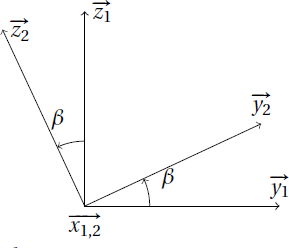
\includegraphics[width=3cm]{figuregeom}
\end{center}
\end{minipage}
\begin{minipage}{0.5\textwidth}
\begin{align*}
\overrightarrow{z}_{0,1}\cdot \overrightarrow{z}_2=\cos\beta\\
\overrightarrow{z}_{0,1}\cdot \overrightarrow{z}_1=1\\
\overrightarrow{z}_{0,1}\cdot \overrightarrow{x}_0=0\\
\overrightarrow{z}_{0,1}\cdot \overrightarrow{x}_1=0\\
\overrightarrow{z}_1\cdot \overrightarrow{y}_2=\sin\beta\\
\end{align*}
\end{minipage}

On trouve alors : 

$
\overrightarrow{z}_0\cdot \vectmc{K}{3}{0}=
m\frac{\dd\left[a\cdot b\cdot \dot{\beta}\cos\beta+a^2\cdot \dot{\alpha}+b^2\cdot \dot{\alpha}\sin^2\beta\right]}{\dd t}
$

$=m\left[a\cdot b\cdot \left(\ddot{\beta}\cos\beta-\dot{\beta}^2\sin\beta\right)+a^2\ddot{\alpha}+b^2\cdot\left(\ddot{\alpha}\sin^2\beta+2\dot{\alpha}\dot{\beta}\sin\beta\cos\beta\right)\right]
$

\end{corrige}
\else
\fi


\subparagraph{} \textit{Dans le cas d'une vitesse de rotation de l'hélice \textbf{2} ($\dot{\beta}$) constante et dans le cas où l'angle $\alpha$ est constant (pas de changement d'orientation de l'éolienne) déterminer l'expression du couple $C_m$ que devrait fournir un moteur placé dans le mat (entre \textbf{0} et \textbf{1}) pour << contrer >> les effets dynamiques du balourd.}

\ifprof
\begin{corrige}
Le théorème du moment dynamique autour de l'axe $\couple{K}{{z}_{0,1}}$ donne :
$
C_m=-m\cdot a\cdot b\cdot \dot{\beta}^2\sin\beta
$.

\end{corrige}
\else
\fi


\ifprof
\else
\end{multicols}
\fi

